\documentclass[14pt,green]{beamer}

\usepackage[utf8x]{inputenc}
\usepackage{default}
\usepackage{ucs}
\usepackage{listings}

\usepackage{fontenc}
\usepackage{graphicx}
\usepackage{wasysym}
\usepackage{listings}
\usepackage{tikz}
\usetikzlibrary{arrows,automata}


\definecolor{mydarkgreen}{RGB}{12,102,29}
\definecolor{darkgreen}{RGB}{0,128,0}
\definecolor{backgreen}{RGB}{133,186,0}
\definecolor{myUNIgreen}{RGB}{0,102,102}

\newcommand{\RedSmile}{\textcolor{red}{\frownie}}
\newcommand{\GreenSmile}{\textcolor{green}{\smiley}}

\setbeamercolor{outlinebox}{fg=white, bg=myUNIgreen}
\setbeamercolor{outlinebox2}{fg=white, bg=mydarkgreen}
\setbeamercolor{item}{fg=myUNIgreen}
\setbeamercolor{uppercol}{fg=white,bg=myUNIgreen}%
\setbeamercolor{lowercol}{fg=black,bg=green}%
\setbeamercolor{block title}{bg=myUNIgreen,fg=white}
\setbeamercolor{block body}{bg=white}%{bg=backgreen}
\setbeamercolor{block_custom}{bg=white, fg=black}
\setbeamercolor{block4title}{bg=white}

 %\setbeamercolor{frametitle}{fg=white}

\author{Alexey A. Mints}
\title[Massive stars in Open Clusters]{First, second and third massive stars in Open Clusters}
\date{XX.12.2010}


\setbeamertemplate{headline}{
  
\includegraphics[height=1cm]{logo.png}\begin{beamercolorbox}[sep=10pt]{outlinebox}
      \hskip1cm \begin{large}\insertsection\end{large}
  \end{beamercolorbox}
}

\setbeamertemplate{footline}
{
  \hbox{%
  \begin{beamercolorbox}[wd=.5\paperwidth,ht=2.25ex,dp=1ex,center]{outlinebox}%
    \usebeamerfont{title in head/foot}A. Mints, \insertdate{}
  \end{beamercolorbox}%
  \begin{beamercolorbox}[wd=.5\paperwidth,ht=2.25ex,dp=1ex,right]{outlinebox2}%
    \usebeamerfont{date in head/foot}
      \insertshorttitle \hspace*{2ex} \insertframenumber{} / \inserttotalframenumber\hspace*{2ex} 
  \end{beamercolorbox}}%
  \vskip0pt%
}

\AtBeginSection[startext]{
\begin{frame}<beamer>
  \frametitle{Outline}
  \begin{center}
    \tableofcontents[currentsection]
  \end{center}
\end{frame}
}

\setbeamertemplate{background}{
\includegraphics[width=\paperwidth,height=\paperheight]{bg.jpg}}

\setbeamertemplate{frametitle}{
\begin{beamercolorbox}[center, rounded=true]{block4title}
%\begin{center}
\insertframetitle
%\end{center}
\end{beamercolorbox}
}


\setlength{\unitlength}{\textwidth}
%\lstset{basicstyle=\tiny, backgroundcolor=\color{white}, frame=single }


\newcommand{\MSun}{M_\odot}
\newcommand{\Mmax}{m_{\mathrm{max}}}
\newcommand{\Mcl}{M_{\mathrm{cl}}}

\begin{document}

\frame[plain]{
  \titlepage
}


\begin{frame}
  \frametitle{Problem description}
  \begin{figure}
   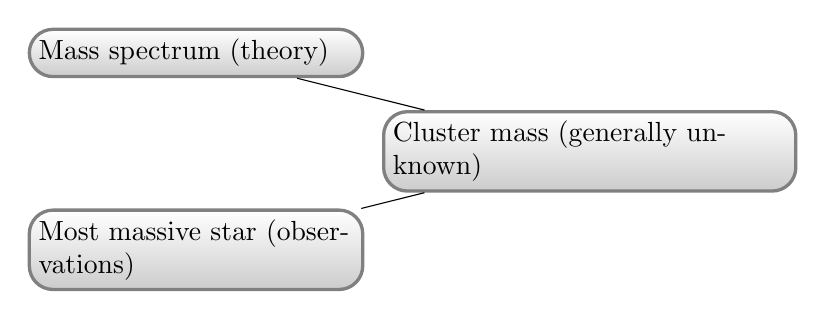
\begin{tikzpicture} [level distance=50 mm,
 every node/.style={ rectangle,minimum size=6mm,rounded corners=3mm,very thick,draw=black!50, top color=white,bottom color=black!20, text width=4cm},
 level 1/.style={sibling distance=25mm,nodes={fill=red!45}},
 level 2/.style={sibling distance=25mm,nodes={fill=red!30}},
]
    \node[text width=5.0cm]{Cluster mass (generally unknown) }[grow=left]
    child{ node{Mass spectrum (theory)} }
    child{ node{Most massive star (observations)} };
   \end{tikzpicture}
  \end{figure}

\end{frame}

\begin{frame}
  \frametitle{Kroupa mass spectrum}
  \begin{beamerboxesrounded}{Spectrum}
  According to Kroupa (2001)
  \begin{align}
  \alpha_0 = +0.30 &\hspace{0.5cm} 0.01 \leq m/\MSun < 0.08, \nonumber \\
  \alpha_1 = +1.30 &\hspace{0.5cm} 0.08 \leq m/\MSun < 0.50, \nonumber \\ 
  \alpha_2 = +2.35 &\hspace{0.5cm} 0.50 \leq m/\MSun < \Mmax. \nonumber 
  \end{align}     
  \end{beamerboxesrounded}
\end{frame}

\begin{frame}
  \frametitle{Ignored effects}
  \begin{beamercolorbox}[center, rounded=true]{block_custom}
   \begin{itemize}
    \item Stellar binarity;
    \item Stellar evolution;
    \item Cluster dynamics;
   \end{itemize}
  \end{beamercolorbox}
\end{frame}

\begin{frame}
  \frametitle{Sampling algorithms}
  \begin{beamercolorbox}[center, rounded=true]{block_custom}
   \begin{itemize}
    \item<+-> Random;
    \item<+-> Constrained;
    \item<+-> Sorted;
   \end{itemize}
  \end{beamercolorbox}
\end{frame}

\begin{frame}
  \frametitle{Distribution for masses of 3 most massive stars}
  \begin{center}
    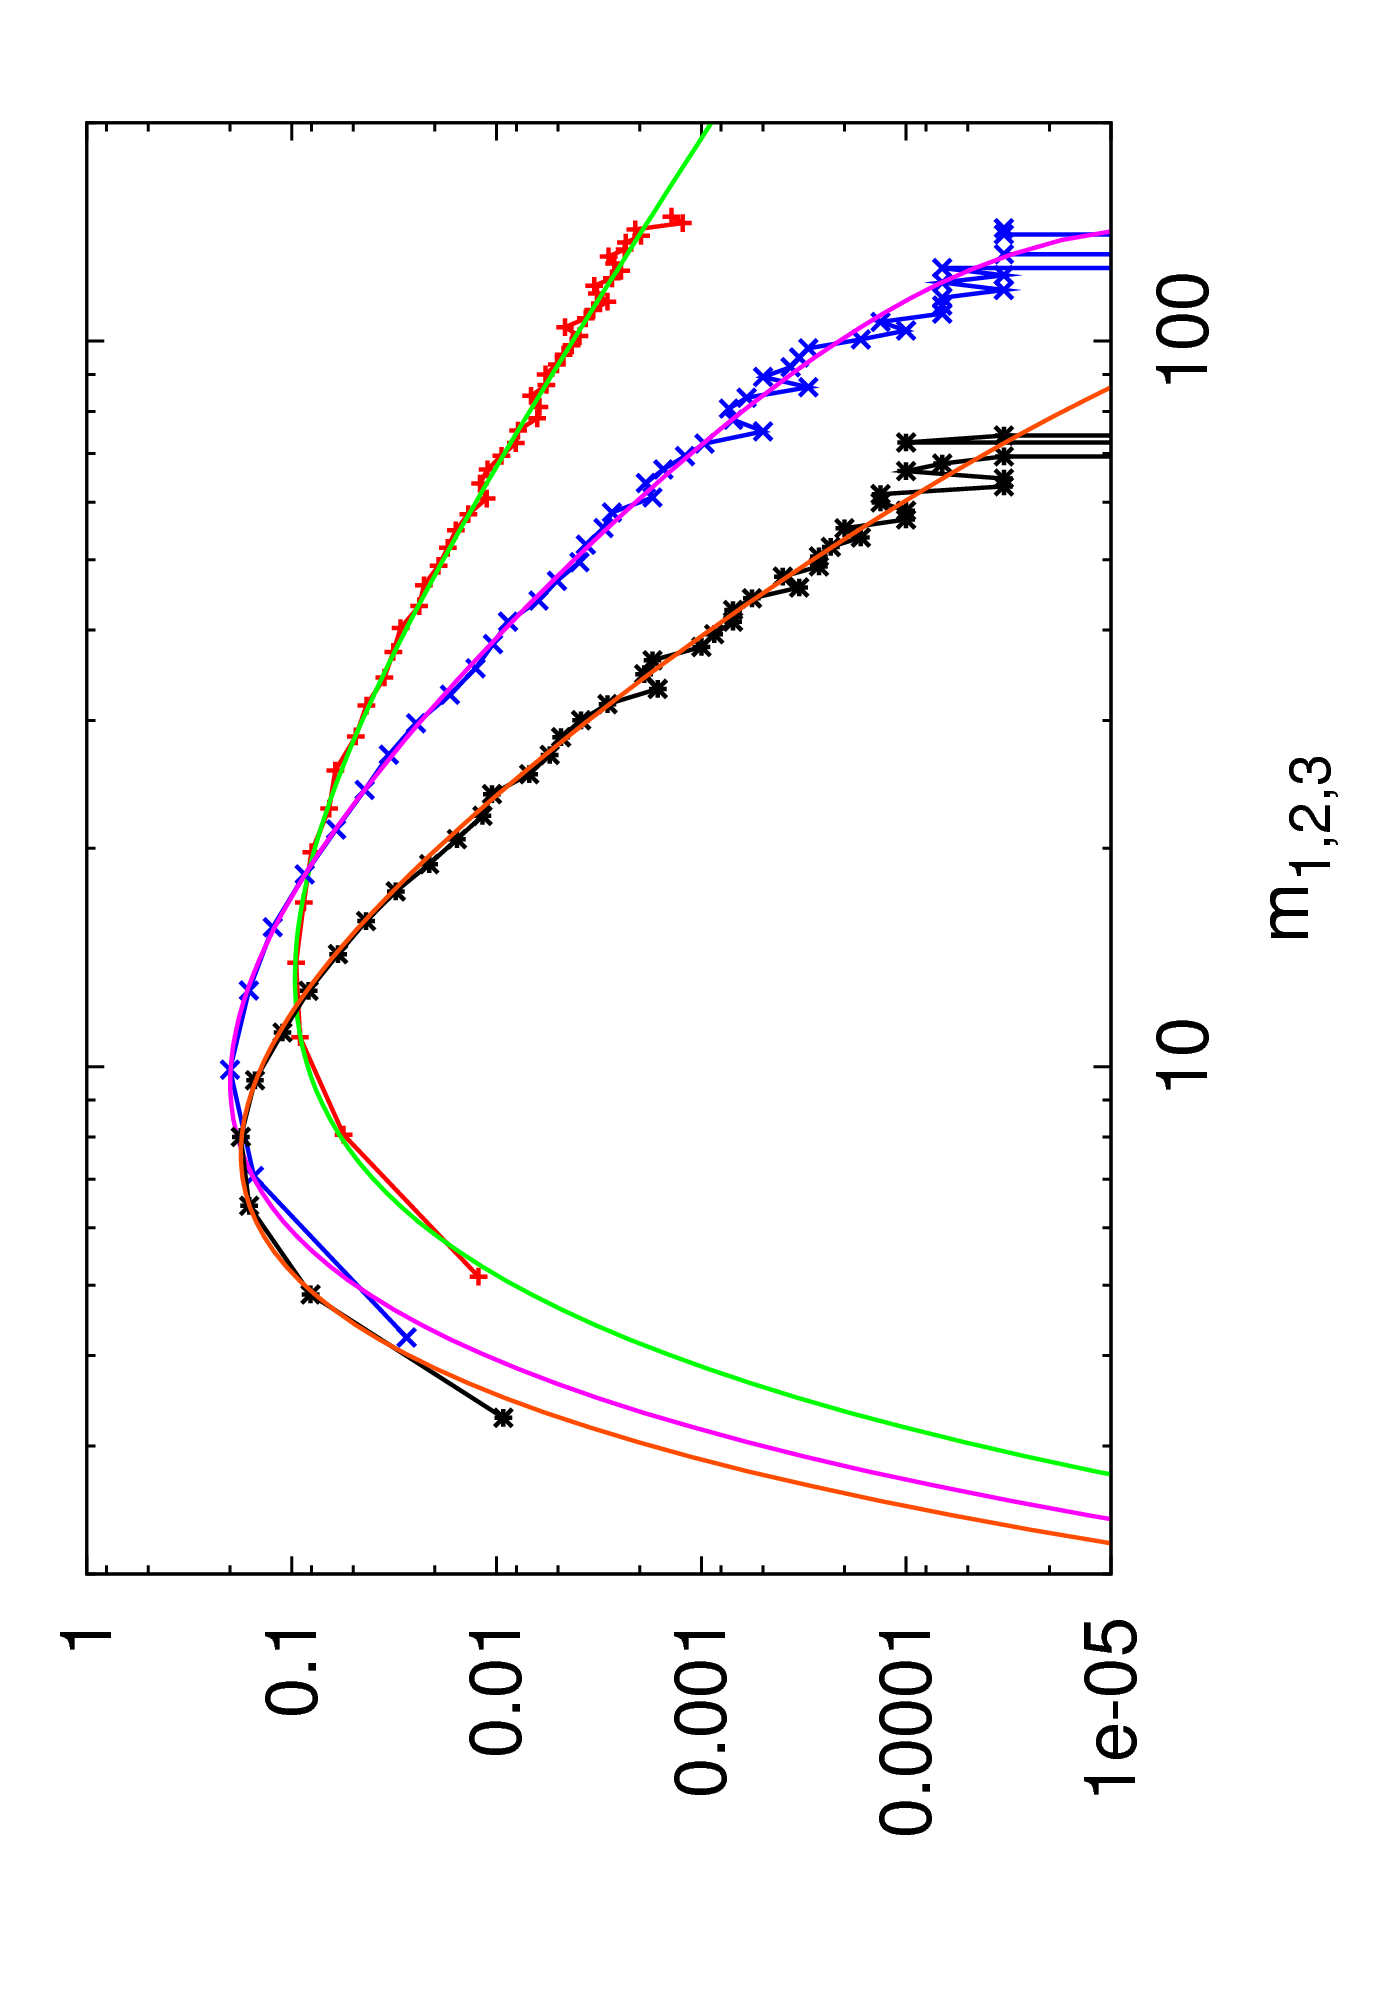
\includegraphics[angle=270, width=0.7\textwidth]{hist_mass.png}                                                                
  \end{center}
\end{frame}
 
\begin{frame}
  \frametitle{Building the estimator function}
  $\Mcl(m_{1,2,3}) = a m_{1,2,3}^b (\Mmax-m_{1,2,3})^c$
\end{frame}
 
\begin{frame}
  \frametitle{$\Mcl(m_i)$}
  \begin{picture}(0.0,0.0) 
     \put(0.1,0.3){    
     \colorbox{white}{
     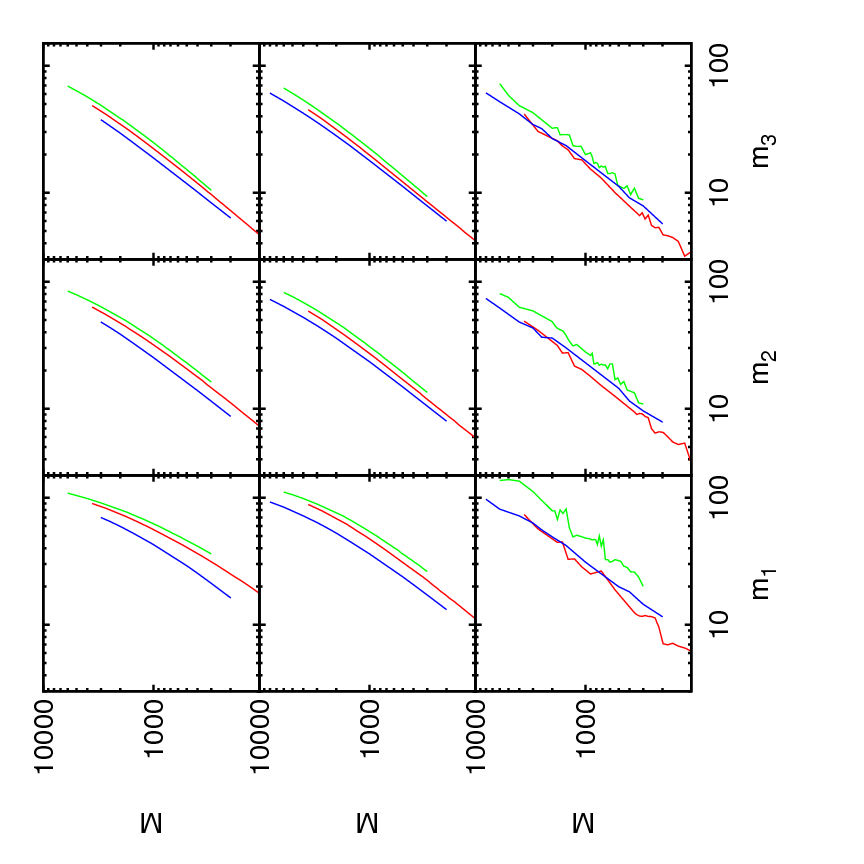
\includegraphics[angle=270, width=0.7\textwidth]{all_estimators.png}                                                                }}
  \end{picture}
\end{frame}

\begin{frame}
  \frametitle{Estimator's error distribution}
  \begin{columns}
    \begin{column}{0.4\textwidth}
       Estimator built on average values. Distribution of estimated $N$ (real value = 1000).
    \end{column}
    \begin{column}{0.6\textwidth}
  \begin{center}
  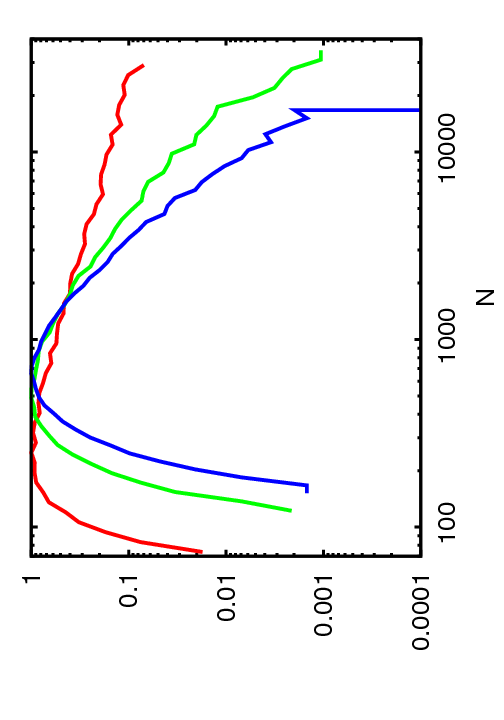
\includegraphics[angle=270, width=1\textwidth]{est_avg.png}                                                             
  \end{center}
    \end{column}
  \end{columns}

\end{frame}

\begin{frame}
  \frametitle{Estimator's error distribution}
  \begin{columns}
    \begin{column}{0.4\textwidth}
       Estimator built on median values. Distribution of estimated $N$ (real value = 1000).
    \end{column}
    \begin{column}{0.6\textwidth}
      \begin{center}
        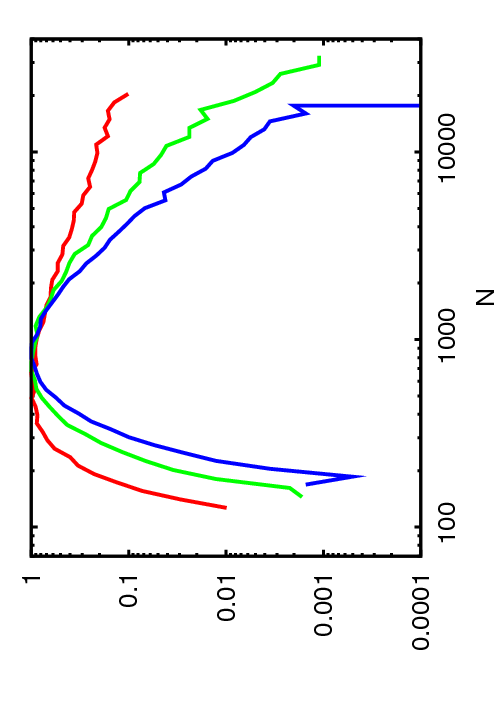
\includegraphics[angle=270, width=0.65\textwidth]{est_med.png}                                                             
      \end{center}
    \end{column}
  \end{columns}
\end{frame}

\begin{frame}
  \frametitle{Estimator's error distribution}
  \begin{columns}
    \begin{column}{0.4\textwidth}
       Estimator built on mode values. Distribution of estimated $N$ (real value = 1000).
    \end{column}
    \begin{column}{0.6\textwidth}
      \begin{center}
        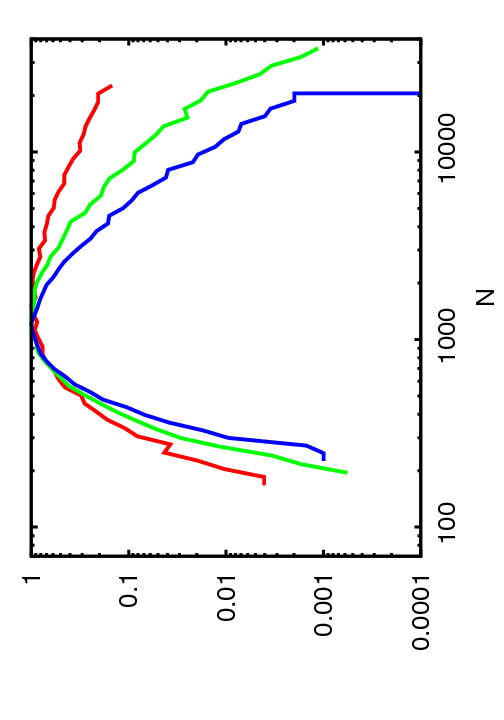
\includegraphics[angle=270, width=0.65\textwidth]{est_max.png}                                                             
      \end{center}
    \end{column}
  \end{columns}
\end{frame}

\begin{frame}
 \frametitle{Conclusions}
  \begin{beamercolorbox}[center, rounded=true]{block_custom}
\begin{enumerate}
 \item Mode or median should be used to build mass estimator;
 \item Errors have power-law tail;
 \item Second or third massive star is a better choice because:
 \begin{itemize}
  \item less affected by the unknown $\Mmax$;
  \item have smaller errors;
 \end{itemize}
\end{enumerate} 
  \end{beamercolorbox}
\end{frame}


\end{document}
